%\documentclass[10pt,a4paper,twoside]{article}
\documentclass[10pt,a4paper]{article}
\usepackage{a4wide}
\linespread{1.359140914229522617680} 
\usepackage[utf8]{inputenc}
\usepackage[german]{babel}
\usepackage{amsmath}
\usepackage{amsfonts}
\usepackage{amssymb}
\usepackage{units} % soll ich das verwenden? oder siunitxs oder garnix?
\usepackage{hyperref}
\usepackage{ulem}
\usepackage{placeins}
\hypersetup{
%    bookmarks=true,
    pdftoolbar=true,
    pdfmenubar=true,
    pdffitwindow=false,
    pdfstartview={FitH},
    pdftitle={Physikalische Grundlagen der Energieübertragung mit Gleich- und Wechselstrom hoher Spannung},
    pdfauthor={Michael F. Sch\"onitzer},
    pdfsubject={HVDC},
    pdfkeywords={HVDC} {HGÜ} {Gleichspannung} {Energieübertragung} {Strom} {Physik},
    pdfnewwindow=true,
    colorlinks=true,
    linkcolor=black,
    citecolor=black,
    filecolor=black,
    urlcolor=blue
}
\setcounter{secnumdepth}{4}

\newcommand{\degree}{$^\circ$}
\newcommand{\q}{\glqq }
\newcommand{\qe}{\grqq }
\newcommand{\rot}{\mathrm{rot\:}}
\newcommand{\tmu}{$\mathrm{\mu}$}
\newcommand{\tOmega}{$\mathrm{\Omega}$}

\usepackage{rotating}
\usepackage[basic]{circ}


\author{Michael F. Schönitzer}
\title{Physikalische Grundlagen der Energieübertragung mit Gleich- und Wechselstrom hoher Spannung }
\begin{document}
\maketitle

\section{Einleitung}
Für die heutige Gesellschaft ist die elektrische Energie von unschätzbarer Bedeutung und trotz der Bemühungen einiger Länder den Stromverbrauch zu reduzieren, steigt er weltweit weiterhin. Begrenzte Ressourcen und wachsendes Umweltbewusstsein auf der anderen Seite führen dazu, dass der Anteil an erneuerbaren Energien steigt. Dadurch wachsen die Anforderungen an die Stromnetze. Dabei wird auch die Die Hochspannungs-Gleichstrom-Übertragung (HGÜ, englisch HVDC) -- die in den letzten Jahrzehnten eher ein Nischendasein geführt hat -- als Alternative und Ergänzung zur Drehstrom-Hochspannungs-Übertragung (DHÜ) wieder entdeckt.
Andererseits ist die DHÜ und der Aufbau eines Stromnetzes ein physikalisch und technisch interessantes Thema, über welche man -- im Vergleich zu ihrer Bedeutung für unser tägliches Leben -- relativ wenig weiß.
In dieser Arbeit möchte ich die physikalischen Grundlagen der Energieübertragung mit Gleich- und Wechselstrom erläutern ohne dafür zu sehr in die technischen Details einzugehen. Die Auswahl wie weit wir in die Einzelheiten der physikalischen Effekte und technischen Umsetzungen eingehen ist subjektiv und hängt auch davon ab wie interessant diese aus physikalischer Sicht sind.

\section{Gleichstrom}
Die Energieübertragung mittels Gleichstrom ist im Grunde relativ einfach und bereits aus der Schule bekannt, wir wollen sie daher hier nur kurz zusammenfassen.
Eine Gleichspannungsquelle liefert einen zeitlich konstanten Potentialunterschied, elektrische Spannung $U$ genannt. Legt man an diese einen ohmschen Widerstand $R$ an, so fließt durch ihn ein zeitlich konstanter Strom
\begin{equation}
I = \frac{U}{R}
\end{equation}
Und leistet an ihm die Leistung
\begin{equation}
P = U \cdot I
\end{equation}
%mehr?


\section{Einphasen-Wechselstrom}\label{wechsel}
Beim Einphasen-Wechselstrom hat man einen Nullleiter und einen Leiter, auf dem eine sinusförmige Wechselspannung mit der Amplitude $U_0$ anliegt:
\begin{equation}
U(t)=U_0 \cdot \cos(\omega t + \varphi)
\end{equation}
Dieser Leiter wird in der Elektrotechnik oft umgangssprachlich als Phase bezeichnet; wir wollen davon hier jedoch nicht Gebrauch machen, da wir physikalisch korrekter den Faktor $\varphi$ als Phasenverschiebung oder kurz Phase bezeichnen werden.

Legt man obige Spannung an einen ohmschen Widerstand R an, so fließt durch ihn der Strom $I(t)= \frac{U(t)}{R} = I_0 \cdot \cos(\omega t + \varphi)$ mit $I_0 = U_0/R$.
Die elektrische Leistung $P$, die an dem Widerstand erbracht wird, wird analog zur Gleichspannungstechnik als Produkt aus Spannung und Strom definiert, dabei beziehen sich jedoch alle drei Größen auf die momentanen Werte:
\begin{equation}
P(t) = U(t) \cdot I(t) \stackrel{\mathrm{\varphi=0}}= U_0 I_0 \cdot \cos^2(\omega t)
\end{equation}
Berechnen wir nun den zeitlichen Mittelwert der Leistung
\begin{equation}\label{eq:Wirkleistung_ohne_phi}
\bar{P}=\frac1T \int\limits_0^T dt\: U_0 I_0 \cos^2 \omega t = \frac12 U_0 I_0 \qquad\mathrm{mit}\; T=2\pi/\omega
\end{equation}
Vergleicht man dies mit der Leistung eines Gleichstroms $P=U\cdot I$, so sieht man, dass eine Gleichspannung mit $U=U_0 / \sqrt2$ und dem daraus folgendem Strom $I=I_0 / \sqrt2$ dieselbe Leistung erbringt.
Deshalb definiert man die Effektivspannung und den Effektivstrom eines Wechselstroms als:
\begin{equation*}
U_{\mathrm{eff}} = \frac{U_0}{\sqrt2} \qquad I_{\mathrm{eff}} = \frac{I_0}{\sqrt2} \qquad \bar{P}=U_{\mathrm{eff}}I_{\mathrm{eff}}
\end{equation*}
Im folgenden werden wir mit $U$ beziehungsweise $I$ die Effektivwerte, mit $U(t)$ beziehungsweise $I(t)$ die Momentanwerte und mit $U_0$ beziehungsweise $I_0$ die Amplituden bezeichnen.


%%% INCLUDE-FILE: Spulen_Kondensatoren.tex %%%

\subsection{Spulen und Kondensatoren im Wechselstromkreis}

\subsubsection{Spulen in Wechselstromkreisen}
Wir betrachten nun einen Wechselstromkreis mit vernachlässigbaren Widerständen, in welcher sich eine Spule befindet. Ein Stromfluss in der Spule führt zu einem Magnetfeld. Da der Stromfluss in der Spule jedoch ständig sein Vorzeichen ändert, wird abwechselnd ein Magnetfeld in die eine Richtung aufgebaut und nach dem Zusammenbrechen dieses dann ein Magnetfeld mit umgekehrter Ausrichtung Richtung aufgebaut.
Die Summe aller Spannungen muss in einem Stromkreis immer Null sein:
$ U_Q + U_{ind} = 0 $.
Wobei $U_Q$ die von der Quelle angelegte Spannung ist und $U_ind$ die durch das Magnetfeld induzierte Spannung in der Spule ist. Letztere berechnet sich durch
\begin{equation}
U_{ind} = - L \cdot \frac{\mathrm dI(t)}{\mathrm dt}
\end{equation}
Daraus folgt durch einsetzen und integrieren
\begin{align}
%U_Q + U_{ind} =& 0 \nonumber \\
%\Rightarrow\;
U_0 \cos \omega t =& L \cdot \frac{\mathrm dI(t)}{\mathrm dt} \nonumber \\ 
\Rightarrow\; I(t) =& \frac{U_0}{L} \int \cos \omega t \mathrm dt = \nonumber \\ 
=& \frac{U_0}{\omega L} \sin \omega t = \nonumber\\
=& I_0 \sin \omega t \qquad mit\qquad I_0 = \frac{U_0}{\omega L}  \nonumber\\
=& I_0 \cos(\omega t - 90^\circ)
\end{align}
Der Strom hinkt der Spannung also um \unit{90}{\degree} hinterher und wir definieren analog zum ohmschen Widerstand den Betrag des induktiven Widerstand als den Quotient zwischen $U_0$ und $I_0$:
\begin{equation}
\left|Z_L\right| = \frac{U_0}{I_0} = \omega \cdot L
\end{equation}
Dies wird auch Induktanz $X_L = \left|Z_L\right| = \omega \cdot L$ genannt.

\subsubsection{Kondensatoren im Wechselstromkreis}
Analog zur Spule, können wir auch die Auswirkung eines Kondensators im stromkreis berechnen. %XXX "Analog"?
Wir beginnen dabei mit der Gleichung
\begin{equation}
U = \frac{Q}{C}
\end{equation}
für den Kondensator und differenzieren diese nach der Zeit:
\begin{equation}
\frac{dU}{dt} = \frac{1}{C}\frac{dQ}{dt} = \frac{1}{C} \cdot I
\end{equation}
Da die angelegte Spannung $U_Q$ der Spannung am Kondensator entspricht, gilt:
\begin{equation}
U_0\cdot \omega \sin \omega t = \frac{1}{C} \cdot I
\end{equation}
und somit
\begin{equation}
I = U_0\cdot \omega C \cos\left( \omega t + 90^\circ\right)
\end{equation}
Während bei einer Spule also der Strom der Spannung um \unit{90}{\degree} hinterher hinkt, eilt er bei einem Stromkreis mit Kondensator um \unit{90}{\degree} voraus. Wir ahnen bereits, dass diese beiden Effekte sich gegenseitig aufheben können.
Auch hier können wir analog zum ohmschen Widerstand den Betrag des kapazitiven Wiederstand definieren:
\begin{equation}
\left|Z_C\right| = \frac{U_0}{I_0} = \frac{1}{\omega C}
\end{equation}
Der Begriff Kapazitanz ist als $X_C = \left|Z_C\right| = -\frac{1}{\omega C}$ definiert.

\subsubsection{Allgemeiner Fall}
Betrachten wir nun einen Wechselstromkreis mit einer Induktivität, einer Kapazität und einem ohmschen Widerstand. Wieder gilt die 2. Kirchhoffsche Regel $\sum U = 0$:
\begin{equation}
U_Q = L \cdot \frac{\mathrm{d}I(t)}{\mathrm{d}t} + \frac{Q}{C} + I(t) \cdot R
\end{equation}
Wir differenzieren nach der Zeit um die Ladung los zu werden:
\begin{equation}
\frac{\mathrm dU_Q}{\mathrm dt} = L \cdot \frac{\mathrm{d^2}I(t)}{\mathrm{d}t^2} + \frac{I(t)}{C} + \frac{\mathrm dI(t)}{\mathrm dt} \cdot R
\end{equation}
Diese Differenzialgleichung können wir mit eines komplexem e-Ansatzes lösen:
Wir lösen diese Differenzialgleichung im Komplexen und betrachten dann den Realteil der komplexen Lösung gemäß Superpositionsprinzip als die physikalisch sinnvollen Lösungen. Zur Lösung  wählen wir den Ansatz:
\begin{equation}
U_Q = U_0 e^{(i\omega t)},	\qquad	I(t) = I_0 e^{i(\omega t-\varphi)}
\end{equation}
Die Wahl von U als komplexe Exponentialfunktion ist deshalb möglich, da der Realteil der komplexen Exponentialfunktion die Kosinus-Funktion ist.
\begin{equation}
Re\left[ U_0 e^{(i\omega t)}\right]  = U_0 \cos{(\omega t)}
\end{equation}
Durch einsetzen in den Ansatz erhalten wir:
\begin{equation}
i\omega U = (- L \omega^2 + i \omega R  + \frac{1}{C}) \cdot I(t)
\end{equation}
Wir definieren analog zum klassischen ohmschen Widerstand den Komplexen Widerstand als Quotient von Spannung und Strom:
\begin{equation}
Z = \frac{U}{I} = R + i ( \omega L - \frac{1}{\omega C})
\end{equation}
Wir stellen diese komplexe Größe nun in Polardarstellung:
\begin{equation}
Z = |Z| \cdot e^{i\varphi}
\end{equation}
mit
\begin{equation}\label{Zpolar}
|Z| = \sqrt{ R^2 + \left( \omega L - \frac{1}{\omega C} \right) }\quad {\mathrm{und}} \quad \tan\varphi = \frac{Im[Z]}{Re[Z]} = \frac{\omega L - \frac{1}{\omega C}}{R}
\end{equation}
Kehren wir nun zur Betrachtung im Reellen zurück um $I_0$ zu bestimmen:
\begin{align}
\nonumber
Re\left[ I \right]
&= Re\left[ \frac{I}{Z} \right] =\\\nonumber
&= Re\left[ \frac{U_0 e^{i\omega t}}{|Z|\cdot e^{i\varphi}} \right] =\\\nonumber
&= \frac{U_0}{|Z|} Re\left[ e^{i(\omega t - \varphi)} \right] =\\
&= \frac{U_0}{|Z|} \cos(\omega t - \varphi) = I_0 \cos(\omega t - \varphi)
\end{align}

Der Tangens der Phasenverschiebung also der Quotient aus Imaginärteil und Realteil des kompexen Widerstands, während die Amplitude der Stromkurve die Amplitude der Spannung durch den Betrag des kompexen Widerstands ist.
Man erkennt in \ref{Zpolar} leicht das die Phasenverschiebung null ist, wenn der Imaginärteil null ist, was für 
\begin{equation}
\omega L = \frac{1}{\omega C}
\end{equation}
der Fall ist. Bei richtiger Wahl von Induktivitäten bzw. Kapazitäten kann man also die Blindleistung einer Kapazität bzw. Induktivität auslöschen.



\subsection{Wirk-, Schein- und Blindleistung und der Leistungsfaktor}
Die Größen Spannung, Leistung und die Phasenverschiebung beschreiben das System vollständig, die Arbeit mit diesen Größen ist jedoch oft kompliziert und aufwändig. Daher zieht man häufig die Beschreibung mit den Größen Wirk-, Schein- und Blindleistung vor, weshalb wir diese hier definieren und näher betrachten wollen.

Die Wirkleistung ist diejenige Leistung, welche real genutzt werden kann, sie wird manchmal auch als aktive Leistung oder Nutzleistung bezeichnet. Sie ist das arithmetische Mittel über die Augenblicksleistung:
\begin{equation}
P = \overline{p} = \overline{U(t) \cdot I(t)}
\end{equation}
Für kosinusförmige Spannungs- und Stromverläufe wird daraus:
\begin{equation}
P = U_0 I_0 \cdot \frac{1}{2\pi} \int\limits_0^{2\pi} \cos\left( \omega t\right) \cos \left(\omega t - \varphi\right)
= \frac{1}{2} U_0 I_0 \cos \varphi
\end{equation}
Dies entspricht natürlich dem unter \eqref{eq:Wirkleistung_ohne_phi} Berechneten, jedoch nun mit Phasenverschiebung. Mit den Effektivwerten wird daraus also:
\begin{equation}
P =  U_{\mathrm{eff}} I_{\mathrm{eff}} \cdot \cos \varphi
\end{equation}
Die Wirkleistung wird in Watt (1 W = 1 V$\cdot$A) gemessen.

Die Scheinleistung ist hingegen das Produkt aus Spannung und Strom ohne Phasenfaktor. Die Verluste und die Beanspruchung der Komponenten verhalten sich, als würde eine Leistung dieser Größe übertragen. Sie stellt die bei einer gewissen Beanspruchung der Leitungskomponenten maximal übertragbare Wirkleistung dar. Sie ist deshalb immer größer oder gleich der Wirkleistung, wobei die Gleichheit für den Fall eintritt, dass die Phasenverschiebung null ist.
\begin{equation}
S = U_{\mathrm{eff}} I_{\mathrm{eff}} \geq P
\end{equation}
Die Scheinleistung ist zwar das Produkt aus Spannung (gemessen in Volt) und Strom (gemessen in Ampere), sie ist jedoch keine Leistung im physikalischen Sinn, deshalb wird sie nicht in Watt, sondern in Voltampere (VA) gemessen.

Als nächstes wollen wir den Leistungsfaktor einführen, er ist das Verhältnis von Wirk- und Scheinleistung:
\begin{equation}
\lambda = \frac{P}{S} \in [0,1]
\end{equation}
In unserem Fall betrachten wir kosinusförmige Spannungen und erhalten somit:
\begin{equation}
\lambda = \cos \varphi
\end{equation}
Wie im Folgenden leicht zu erkennen, beeinflusst der Leistungsfaktor den Wirkungsgrad der Komponenten:
\begin{equation}
\eta = \frac{P}{P+P_V} = \frac{\frac{P}{S}}{\frac{P}{S}+\frac{P_V}{S}} = \frac{\lambda}{\lambda + p_V} \qquad \mathrm{(mit}\;P_V\;\mathrm{als\: Verlustleistung)}
\end{equation}
Sinkt also der Leistungsfaktor, so reduziert sich dadurch auch der Wirkungsgrad einer Komponente.
Sofern nicht anders angegeben, bezieht sich der angegebene Wirkungsgrad einer Komponente immer auf einen Leistungsfaktor von 1, also der Situation, dass Strom und Spannung phasengleich verlaufen.
Hat man einen Phasenverschiebung ungleich null, so ist der Wirkungsgrad teils bedeutend geringer.
Für einen Leistungsfaktor von Null -- also eine Phasenverschiebung von 90\degree -- wird das System zwar von der Scheinleistung S beansprucht und es entstehen Verluste, es findet aber keinerlei Energieübertragung statt und der Wirkungsgrad ist null.
Der Leistungsfaktor kann auch als die Wurzel des Verhältnisses der minimal notwendigen und den tatsächlichen Verlusten ausgedrückt werden:
\begin{equation}
\lambda = \sqrt{\frac{P_{V\:min}}{P_V}}	% Herleitung?
\end{equation}
ein Leistungsfaktor von 0.8 würde also beispielsweise bedeuten, dass die Verluste 56\% größer sind als nötig.

Als dritte Leistungs-Größe wollen wir noch die Blindleistung $Q$ einführen.
%Diese Größe steht auf der Wirkleistung im Zeigerdiagramm orthogonal. %XXX Zeigerdiagramme hab ich noch nicht; Grafik?
%Sie lässt sich mit Pythagoras berechnen:
Die Blindleistung ist die Komponente der Scheinleistung, welche keine Arbeit verrichtet – also das gegenteil zur Wirkleistung. Sie ergibt sich im allgemeinen Fall aus $S^2=P^2+Q^2$ zu:
\begin{equation}
Q = \sqrt{S^2-P^2} = S \sqrt{1-\lambda^2} = P \frac{\sqrt{1-\lambda^2}}{\lambda}
\end{equation}
Für kosinusförmige Ströme wird sie zu:
\begin{equation}
Q = S \sqrt{1-\cos^2 \varphi} = S sin \varphi = U_{\mathrm{eff}} I_{\mathrm{eff}} sin \varphi
\end{equation}
Die Blindleistung trägt nicht zu Energieübertragung bei, sondern belastet nur die Komponenten. Sie ist ebenfalls keine physikalische Leistung, man misst sie in Voltampere reaktiv (Var\footnote{Var wird als Wort ausgesprochen.} oder älter VAr).
Die Blindleistung kann positiv oder negativ sein, per Konvention nimmt man sie als positiv an der Last an, wenn die Last induktiv ist. Dies ist vorteilhaft, da die meisten Lasten induktiv sind und man sie somit als Verbraucher von Wirk- und Blindleistung ansehen kann. Kondensatoren kann man als Quellen von Blindleistung ansehen.\cite{Harrison}

Zum Abschluss wollen wir noch die komplexe Leistung, auch Leistungsvektor oder komplexe Scheinleistung genannt, einführen: $\underline{S} = P+i Q$. Die oben eingeführte Scheinleistung $S$ ist dabei der Betrag der komplexen Scheinleistung $\underline{S}$.

% wo anders hin verschieben, da auch bei Gleichspannung!?
\subsection{Ohmscher Verlust}
Fließt ein Strom $I$ mit der Spannung $U$ durch einen ohmschen Widerstand, so wird dabei die elektrische Leistung
$P_V = U' \cdot I = R \cdot I^2$
in Wärme umgesetzt, wobei $U'$ die an dem Widerstand abfallende Spannung ist.
Da die übertragene Leistung $P=U \cdot I \cdot \cos(\varphi)$ ist, folgt für die Verlustleistung
\begin{equation}\label{eq:Verlust}
P_V = \left(\frac{P}{U \cdot \cos\varphi}\right)^2\cdot R
\end{equation}
Bei der Übertragung von Energie stellt das Kabel einen Widerstand dar und die Verlustleistung soll möglichst minimiert werden. Da der Widerstand nur bedingt verringert werden kann, erhöht man die Spannung und verringert somit den Stromfluss. Eine Leitung mit einer Spannung von 110\,kV hat einen Verlust von etwa 6\% je 100\,km, eine Leitung mit 800\,kV verliert auf der selben Distanz nur etwa 0.5\%.

Andererseits sehen wir, dass der Ohmsche Verlust mit steigender Phasenverschiebung ins Unendliche steigt. Daher ist man bemüht diese möglichst gering zu halten. Wie wir gesehen haben, ist dies durch Kompensation mit Spulen beziehungsweise Kondensatoren möglich.

Der Gleichstromwiederstand eines Materials hängt auch von der Temperatur $\vartheta$ des Leiters ab. Mann rechnet deshalb meist mit dem Widerstand $R_{20}$, den das Material bei einer Temperatur von $20^\circ C$ hat, und einem Temperaturbeiwert $\alpha_{20}$, der angibt wie stark der Widerstand mit der Temperatur steigt:
\begin{equation}
R_\vartheta = R_{20} \cdot \left[ 1 + \alpha_{20} \cdot \left( \vartheta - 20^\circ C \right) \right]
\end{equation}
Beide Werte sind empirisch bestimmte Materialkonstanten.

%%% INCLUDE-FILE: Skineffekt.tex %%%

\subsection{Skin-Effekt}
Der Widerstand einer Stromdurchflossen Leitung hängt neben der Länge und dem Material auch vom Querschnitt des Leiters ab. Dabei rechnet man in der Gleichstromtechnik mit
\begin{equation}
R = \rho \cdot l \cdot A
\end{equation}
Bei Wechselstrom kommt es jedoch zum sogenannten Skin-Effekt: der Stromfluss im Leiter wird nach außen verdrängt, es fließt also in den Äußeren Schichten wesentlich mehr Strom als in den inneren Schichten. Dieser Effekt ist um so stärker, je höher die Frequenz der Spannung ist. Bei den 50 Hz beziehungsweise 60 Hz die bei den Energienetzen üblich sind, ist der Effekt vergleichsweise schwach. Erst bei deutlich höheren Frequenzen wird der Effekt so stark, dass er der Stromfluss sich praktisch vollständig auf eine dünne Schicht (Haut) beschränkt -- woher der Effekt seinen Namen hat.

Die Stromdichte im Leiter nimmt nach außen hin gemäß
\begin{equation}
J = J_S e^{-\frac{d}{\rho}}
\end{equation}
ab, wobei $J_S$ die Stromdichte am Rand ist und die sogenannte äquivalenten Leitschichtdicke $\rho$ die Tiefe ist, in welcher die Stromdichte auf $1/e$ abgesunken ist. Für Kupfer beträgt der Wert von $\rho$ 9,38 mm (50 Hz), beziehungsweise 8,57 mm (60 Hz).

Der Skineffekt wurde 1873 von J. C. Maxwell vorhergesagt und 1885 von D. E. Hughe erstmals experimentell nachgewiesen\cite{BergmannSchaefer}.

Zum Verständniss des Effekts betrachten wir ein Flächenelement ds dr im Drahtinneren.
An dem Draht liegt eine Spannung an, welche also ein Elektrische Feld im Draht erzeugt
Andererseits fließt duch den Draht ein Strom, durch welchen ein Magnetische Feld aufgebaut wird.
Da es sich um Wechselstrom handelt, ändert das Magnetfeld ständig seine Richtung und Stärke, wodurch ein elektrisches Wirbelfeld induziert wird.
Auf der der Achse zugewandten Seite ist das induzierte Elektrische Feld dem äußerem Feld entgegengerichtet, auf der der Achse abgewandten Seite gleichgerichtet.
Das resultierende elektrische Feld und somit auch die Stromdichte muss also von innen nach ausen zunehmen.

Die genaue Herleitung des Skineffektes ist relativ kompliziert, Sie kann in einem Lehrbuch der Elektrodynamik nachgeschlagen werden. % zum beispiel…
Wir wollen hier lediglich eine einfache Herleitung der Eindringtiefe beschreiben.
Wir starten dabei mit den Maxwellgleichungen, genauer gesagt mit dem Induktionsgesetz von Faraday und dem erweiterten ampèreschen Gesetz:
\begin{align}
\nabla \times \mathbf{E} &= -\frac{\partial \mathbf{B}}{\partial t} \qquad &\mathrm{(Induktionsgesetz\ von\ Faraday)} \\
\nabla \times \mathbf{H} &= \mathbf{j} + \frac{\partial \mathbf{D}}{\partial t} \qquad &\mathrm{(Erweitertes\ amp\grave{e}resches\ Gesetz)}
\end{align}
Die Elektrische Flussdichte $D$ hängt mit der elektrischen Feldstärke $E$ zusammen:
\begin{equation}
\mathbf D = \epsilon_0 \epsilon_r \mathbf{E}
\end{equation}
Da die elektrisches Feldstärke von der Spannung abhängt, stellt auch sie eine Trigonometrische Funktion von $\omega t$ dar, die Ableitung wird somit zu:
\begin{equation}
\mathbf{\dot{D}} = \omega \epsilon_0 \mathbf{E}
\end{equation}\footnote{Warum wir hier das $\epsilon_r$ ignorieren können, habe ich leider nicht herausgefunden.}
Die Stromdichte j ergibt sich aus der Elektrischen Feldstärke und der elektrische Leitfähigkeit nach dem ohmschen Gesetz zu $j = \rho \mathbf E$. Daraus sehen wir, dass für $\omega \ll \frac{\rho}{\epsilon} \approx 10^{18} s^{-1}$ $\mathbf{\dot{D}}$ vernachlässigbar klein gegenüber $j$ ist.

Die magnetische Flussdichte $\mathbf B$ hängt analog mit der magnetischen Feldstärke $\mathbf H$ zusammen:
\begin{equation}
\mathbf B = \mu_0 \mu_r \mathbf H
\end{equation} 
Woraus folgt:
\begin{equation}
\mathbf{\dot{B}} = \mu_0 \mu_r \mathbf{\dot{H}}
\end{equation} 
Auf der anderen Seite folgt aus obiger Schreibweise des Ohmschen Gesetzes das 
\begin{equation}
\rot \mathbf E = \frac{1}{\rho} \rot j
\end{equation}
Damit folgt:
\begin{equation}
\rot \mathbf H = j \qquad
\rot \mathbf E = \frac{1}{\rho} \rot j = \mu_0 \mu_r \mathbf{\dot{H}}
\end{equation}
Woraus wird durch Elimination von $H$
\begin{equation}
\rot\rot j = \rho \mu_0 \mu_r \dot{j}
\end{equation}
Die zeitliche Ableitung entspricht einer Multiplikation mit $\omega$, die zweimalig räumliche ableitung (rot rot) einer zweimaligen Multiplikation mit der reziproken Schicht dicke, auf der der Strom auf $\frac{1}{e}$ abfällt, und wir erhalten:
\begin{equation}
\frac{1}{d^2} j \approx \omega \rho \mu_r \mu_0 j
\end{equation}



% wo anders hin verschieben, da auch bei Gleichspannung!?
\subsection{Koronaentladung} %QUELLEN
Liegt an einem vergleichsweise dünnem Kabel eine hohe Spannung an, so herrschen in seiner unmittelbaren Nähe sehr hohe elektrische Felder. Sind diese Feldstärken größenordnungsmäßig vergleichbar mit der Durchschlagfestigkeit von Luft (der Feldstärke ab der es zu einem Spannungsdurchschlag kommt), so wird die Luft ionisiert, was zu Verlusten führt. Bei Wechselspannung ist dieses Problem besonders groß, da die Scheitelspannung $U_0$ um den Faktor $\sqrt{2}$ größer als die Effektivspannung ist, es kommt also im Moment, wenn der Scheitelwert erreicht wird, auch bei geringeren Effektivspannungen bereits zur Koronaentladung. Dies betrifft insbesondere die 400-kV-Schiene (Scheitelspannung von 566 kV) und macht Übertragungen von mehr als 500 kV per Freileitung fast unmöglich.%Quelle, Richtig?

Die ist die Koronaentladung ist bei negativ geladen Leitern wesentlich höher als bei positiv geladenen\cite{Padiyar}, diese große Asymmetrie kann durch den Massenunterschied zwischen den Elektronen und den positiv geladenen Ionen. %Quelle

\section{Drehstrom}
Beim Dreiphasen-Wechselstrom, auch Drehstrom genannt, hat man drei stromführende Leiter, an welchen je eine kosinusförmige Spannung mit gleiche Frequenz, aber jeweils 120\degree\  Phasenverschiebung anliegt.
Die Notwendigkeit eines zusätzlichen Nullleiters entfällt, da die drei Spannungen addiert sich aufheben.
Die Spannung zwischen einer beliebigen Leitung und einem Nullleiter wird als Sternspannung bezeichnet,
die Spannung zwischen zwei beliebigen Spannungen als verkettete Spannung. Es gilt:
\begin{equation}
U_{\mathrm{eff},\:\mathrm{verkettet}} = \sqrt{3} \cdot U_{\mathrm{eff},\:\mathrm{Stern}}
\end{equation}
Die Effekte und Aussagen aus Kapitel \ref{wechsel} gelten ansonsten analog auch für Drehstrom, weshalb wir sie nicht wiederholen wollen.

Während Privathaushalte nahezu ausnahmslos einphasigen Strom verwenden, verwendet man in der Industrie und vor allem in der Stromerzeugung und beim Stromtransport nahezu ausschließlich Dreiphasen-Wechselstrom. %Quelle
Dies bringt mehrere Vorteile:
\begin{itemize}
\item Die durch Einphasen-Wechselstrom übertragene Leistung pulsiert mit der doppelten Netzfrequenz, die von Drehstrom übertragene Leistung ist hingegen zeitlich konstant. Dadruch haben insbesondere Motoren ein zeitlich konstantes Drehmoment und laufen somit ruhiger.\cite{Herold}\cite{Harrison}
\item Bei gegebenem Materialaufwand hat eine dreiphasige Maschine eine höhere Leistung.\cite{Harrison} %warum?
\item Bei gleichem Materialaufwand kann ein dreiphasiges Stromnetz mehr Leistung übertragen – der sogenannte Kupferwirkungsgrad ist ein drittel höher.\cite{Herold}
\end{itemize}

\section{Elektrische Netze}
\subsection{Leitungen}

\subsubsection{Leitungsbeläge}
Bisher haben wir die Grundlagen der Gleich- beziehungsweise Wechselstromtechnik im allgemeinen kennen gelernt.
Insbesondere bei der Betrachtung von Blindleistungen geht man dabei meist davon aus,
dass ein Verbraucher durch den Einsatz von Spulen oder Kondensatoren Blindleistung erzeugt.
Wir interessieren uns jedoch für die Energienetze und hier kommt ein wichtiger Punkt hinzu:
Auch die Leitungen selbst haben einen Widerstand, eine Kapazität, eine Induktivität, sowie die noch einzuführende Ableitung.
Diese bezeichnet man auf die Länge bezogen als Widerstand-, Kapazitäts-, Induktivitäts- und Ableitungsbeläge und fasst sie unter dem Begriff der Leitungsbeläge zusammen.

Zunächst sei noch die Ableitung eingeführt: Die Ableitungsbeläge beschreiben die Verluste durch unvollständige Isolation des Kabels. Die Ableitung wird in Siemens\footnote{Eine alternative, ältere Bezeichnung für das Siemens ist das Mho (Ohm Rückwerts gelesen) $\mho$ } gemessen, was den Kehrwert der Einheit Ohm darstellt:
\begin{equation}
\mathrm{[S]} = \frac{1}{\Omega} = \frac{A}{V}
\end{equation}
Die Ableitungsbeläge folglich in Siemens pro Meter.
Die Ableitung ist dank moderner Isolationstechnik deutlich geringer als die Ohmschen Verluste.

Bei der Betrachtung der Leitungsbeläge und der daraus folgenden Anforderungen an die Leitungen muss man zwischen drei unterschiedlichen Leitungstypen unterscheiden: Freileitungen, Erdkabel und Unterseekabel %  Begriff richtig?

\subsubsection{Freileitungen}
Der überwiegende Teil der Hochspannungs-Energieverteilung geschieht mit Freileitungen.
Dabei werden nicht isolierte Leiterseile an Isolatoren an etwa 50 Meter hohen und etwa 400 Meter voneinander entfernten Hochspannungsmasten aufgehängt. % Werte für GB
In Deutschland gibt es Freileitungen mit bis zu 380 kV in anderen Ländern auch bis 1000 kV und Anlagen mit bis zu 2 MV sin geplant\cite{Flosdorff}.
Es gibt unterschiedliche Arten und Bauweisen von Freileitungsmasten, auf die wir hier nicht näher eingehen wollen. Wichtig sind für uns lediglich die sich dadurch ergebende Anzahl und Anordnung der Leiterseile, deren Bodenhöhe und Abstand zu einander.

Die Spitze der Masten tragen ein Erdseil, welches die Leiterseile vor Blitzschlag schützen, indem Sie ein Schutzraum bilden. Er wird näherungsweise durch den Zwischenraum zwischen zwei den Boden und das Erdseil tangierenden Kreisen mit doppelter Masthöhe als Radius beschreiben. Die Masten sind derartig gebaut, dass die die Leiterseile sich in diesem Schutzraum befinden. Um bei – bei besonders hohen Spannungen nötige – weiten Travernen den Mast nicht zu hoch bauen zu müssen, kann man durch Verwendung von zwei statt nur einem Erdseil den Schutzraum vergrößern.

Bei den Leiterseilen handelt es sich meist um Verbundseile mit einem Kern aus Stahl, der die mechanische Stabilität gewährleistet, umgeben von Aluminiumleitern. Aluminium hat zwar im Bezug auf das Volumen einen höheren Widerstand als Kupfer, im Bezug auf das Gewicht leitet Aluminium hingegen besser. Ein typisches 650-A-Leiterseil besteht aus 7 Stahl- und 54 Aluminiumadern, die jeweils einen Durchmesser von 3 mm haben.\cite{Harrison}.
Moderne Leiterseile bestehen oft ganz aus einer Aluminiumlegierung und haben dadurch einen höheren Stromtragefähigkeit, einen geringen ohmschen Widerstand und müssen weniger gewartet werden\cite{Harrison}.
%% Skineffekt
Bei höheren Spannungen verwendet man statt einer dicken mehrere dünnere Leiter pro Phase seil in geringem Abstand. Dadurch sind die Randfeldstärken\footnote{Die Randfeldstärke darf zur Vermeidung von Koronaentladung nicht größer als 17 kV/cm werden.\cite{Flosdorff}} und die Induktivität geringer und durch die bessere Kühlung aufgrund der größeren Oberfläche kann ein größerer Strom geführt werden. Man spricht hier von Bündelleitern.
Seit einigen Jahren stattet man vor allem die Erdseile, aber auch die Leiterseile mit Lichtwellenleitern zur Datenübertragung aus. Diese dienten zunächst der innerbetrieblichen Fernüberwachung- und -steuerung, wird heute jedoch vor allem auch für privat genutzte Telefonnetze verwendet.\cite{Flosdorff}
% Durchhang, entfernung, Last, Wetter, etc. ?

\begin{figure}[tbhn]
\begin{center}
\noindent
\label{Ersatzschaltbildfreileitung}
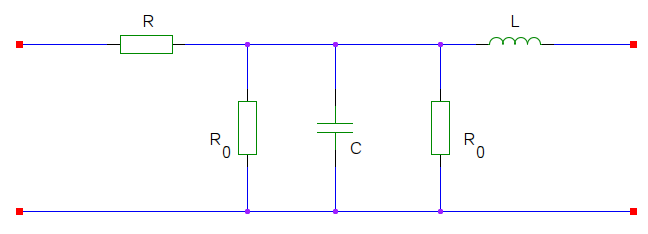
\includegraphics[scale=0.5]{freileitung.png}
\end{center}
\caption{Ersatzschaltbild einer Freileitung} %mehr
\end{figure}

In Abbildung \ref{Ersatzschaltbildfreileitung} ist ein Ersatzschaltbild für eine Einphasige Leitung mit den Leitungsbelägen gezeichnet.
% Alternativ: π-Glied
Dabei ist R der serielle Widerstand, L die serielle Induktivität, C die Parallele Kapazität und $R_0$ der Ableitungswiederstand. Für die genaue Betrachtung muss man sich dieses infinitesimal Klein, unendlich oft hintereinander geschaltet vorstellen, für kurze Leitungen (unter 100 km Länge), kann man es jedoch näherungsweise auf eine derartige Schaltung reduzieren. Außerdem sind im allgemeinen die Induktivitäten nicht notwendigerweise zeitlich konstant.\cite{Flosdorff}
Typische Werte für den Widerstand, die Induktivität und Kapazität findet man in Tabelle \ref{Tabfreileitung}. Der Wert für die Ableitungsbelag hängt stark von äußeren Faktoren, wie den Umgebungsbedingungen und dem Verschmutzungsgrad der Isolatoren ab. Ein typische Wert ist $200\,M\Omega m^{-1}$.\cite{Harrison} Die Ableitungsverluste sind also meist deutlich geringer als die seriellen ohmschen Verluste, weshalb man sie in den meisten Betrachtungen ignorieren kann. Wie wir sehen ist eine Freileitung weitgehend induktiv. % sieht man garnicht

\setlength{\tabcolsep}{10pt}
\renewcommand{\arraystretch}{1.5}
\begin{table}[tbhn]
\begin{center}
\noindent
\begin{tabular}{|c|ccc|}
\hline 
Leitung & 132 kV ($1\cdot 175\ mm^2$) & 275 kV ($2\cdot 400\ mm^2$) & 400 kV ($4\cdot 400\ mm^2$) \\ 
\hline 
R & 0,178 $\Omega$ & 0,039 $\Omega$ & $0,02 \Omega$ \\ 

$X_L$ & 0,40 $\Omega$ & 0,32 $\Omega$ & 0,278 $\Omega$ \\ 

$X_C$ & 350 k$\Omega$ & 275 k$\Omega$ & 245 k$\Omega$ \\ 
\hline 
\end{tabular} 
\end{center}
\caption{bla} %fehlt
\label{Tabfreileitung}
\end{table}

%%% Induktivität %%%
\paragraph{Induktivitätsbelag}

\begin{figure}[tbhn]
\begin{center}
\noindent
\label{leitungsreaktanz} 
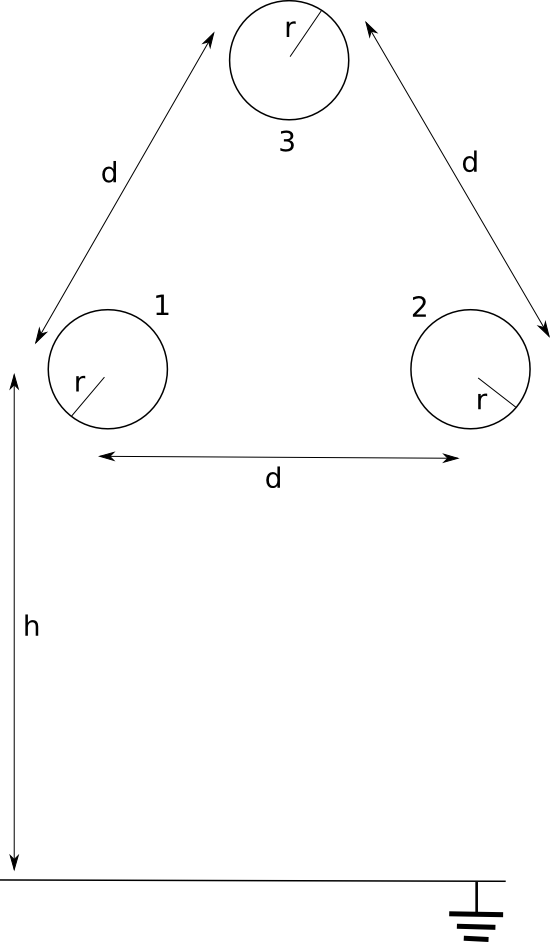
\includegraphics[scale=0.5]{leitungsreaktanz.png}
\end{center}
\caption{bla} %fehlt
\end{figure}

Fließen Wechselströme durch mehrere nebeneinander liegende Leiter so wird durch Selbstinduktion und Gegeninduktion eine Wechselspannung induziert.
%bla, von wegen kan als selbstinduktion gesehen werden
Die Induktivität eines Leiters $v$ hängt wie folgt mit dm magnetischem Fluss an dessen Position zusammen:
\begin{equation}
L_v = N_v \frac{\Phi_v}{i_v}
\end{equation}
Laut \cite{Flosdorff}\cite{Moeller} % besser [42] dort
ist $N_v = 1$, somit müssen wir um die Induktivität zu berechnen den magnetischen Fluss berechnen, welchen sich aus den Flüssen aller Leiter zusammensetzt. Es gilt also das Gleichungssystem:
\begin{equation}\label{SummePhi}
\Phi_v = \sum_k \Phi_{vk}
\end{equation}
%Da Feldlinien stets von einer Quelle ausgehen und in einer Senke enden, benötigen wir noch eine äußere Feldbegrenzung. %realy?
Zur Berechnung der Flüsse führen wir einen Zylinder mit sehr großem, aber endlichem Radius $r_a$ und den Leiter $v$ als Mittelpunkt als Feldbegrenzung ein. Die Rechtfertigung dafür werden wir später sehen.
Der Fluss den der Leiter selbst erzeugt ist laut \cite{Moeller}\cite{Flosdorff} % beide zitieren?
\begin{equation}
\Phi_{vv} = \frac{\mu_0l}{2\pi} \left( \ln\frac{r_a}{r_v} + 0,25 \right) i_v
\end{equation}
Der Fluss im Leiter $v$ der von einem Leiter $k$ erzeugt wird ist das Integral des Magnetfelds über die Fläche zwischen Leiter und Begrenzungszylinder:
\begin{equation}
\Phi_{vk} = \int_A B_k dA = \int\limits_{x=d_{vk}}^{x=r_a} \frac{\mu_0i_k l}{2\pi x}dx =
\frac{\mu_0l}{2\pi}\ln\left(\frac{r_a}{d_{vk}}\right) i_k
\end{equation}
Setzt man dies in Gleichung \ref{SummePhi} ein, so erhält man:
\begin{equation}
\Phi_v = \frac{\mu_0l}{2\pi} \left[ \left( \ln\frac{r_a}{r_v} +0,25\right) i_v + \sum_{k\neq1}\ln\frac{r_a}{d_{vk}} i_k \right]
\end{equation}
Wir beziehen den Fluss auf die Länge der Leitung und zeihen $r_a$ raus:
\begin{equation}
\Phi'_v = \frac{\mu_0}{2\pi}
 \left[
   \ln r_a \sum i_k +
   \sum_k \left( \ln\frac{1}{d_{vk}} i_k +
   0,25 \: \delta_{ik} \right)
 \right]
\quad mit \: d_{v1}:=r_v
\end{equation}
Die Summe aller Leiterströme muss immer null sein $\sum i_k=0$ und somit verschwindet der erste Term und die Gleichung ist unabhängig von $r_a$. Das Gleichungssystem für die Flüsse wird somit zu:
\begin{equation}
\Phi'_v = \sum_k a_{vk}i_k
\end{equation}
mit den Koeffizienten:
\begin{equation}
a_vv = \frac{\mu_0}{2\pi} \left( \ln\frac{1}{r_v} + 0,25 \right) \qquad und \qquad a_{vk} = a_{kv} = \frac{\mu_0}{2\pi} \ln\frac{1}{d_{ik}}
\end{equation}
Betrachten wir zunächst ein \textbf{Zweileitersystem}. Das obige Gleichungssystem reduziert sich auf:
\begin{align}
\Phi'_1 &= a_{11}i_1 + a_{12}i_2 \\
\Phi'_2 &= a_{21}i_i + a_{22}i_2
\end{align}
Dabei ist $i_2 = -i_1$ und $d_{12} = d_{21} = d$. Die Induktivität errechnet sich nun einfach zu:
\begin{equation}
L'_1 = a_{11} - a{12} = \frac{\mu_0}{2\pi}\left(\ln\frac{1}{r_1}+025\right)-\frac{\mu_0}{2\pi}\ln\frac{1}{d} = 
\frac{\mu_0}{2\pi}\left(\ln\frac{d}{r_1}+025\right)
\end{equation}
und gleichfalls für Leiter 2. In der Regel sind die beiden Leiterradien gleich, wodurch beide Leiter die selbe Induktivität haben – was aus Symmetriegründen selbst verständlich war. Will man die Induktivität nicht auf die Leiterlänge sonder auf die Leitungslänge beziehen, so muss man die Induktivität verdoppeln, da man zwei Leiter hat – man erhält also schließlich:
\begin{equation}
L' = \frac{\mu_0}{\pi}\left(\ln\frac{d}{r_1}+025\right)
\end{equation}

Ein weiterer wichtiger Sonderfall ist die symmetrische Dreileiteranordnung, bei welcher alle drei Leiterabstände sowie Leiterradien jeweils gleichgroß sind: $d_1=d_2=d_3:=d$ und $r_1=r_2=r_3:=r$ und somit $a_{12}=a_{23}=a_{13}$. Auch hier sind die Induktivitäten der Leiter gleich groß. Wir errechnen für den ersten Leiter:
\begin{equation}
\Phi'_1 = a_{11}i_1+a_{12}i_2+a_{13}i_3 = a_{11}i_1+a_{12}\left(i_2+i_3\right) = \left(a_{11}-a_{12}\right)i_1
\end{equation}
und daraus:
\begin{equation}
L'_1 = \frac{\Phi'_1}{i_1} = a_{11}-a_{12} = \frac{\mu_0}{2\pi}\left(\ln\frac{1}{r}+0,25-\ln\frac{1}{d} \right) =
\frac{\mu_0}{2\pi}\left(\ln\frac{d}{r}+0,25 \right)
\end{equation}
Ist das Drehstromnetz gleichphasig belastet, so addieren sich die Spannungen und Ströme zu null und es genügt einphasig zu rechnen, da keine Rückführung mehr nötig ist. Die auf die Leitungslänge gerechnete Induktivität ist also:
\begin{equation}\label{Induktivitaet3}
L' = L'_1 = \frac{\mu_0}{2\pi}\left(\ln\frac{d}{r}+0,25 \right)
\end{equation}
Laut \cite{Harrison} gilt diese Gleichung nur für $h\gg d$ – ist dies nicht gegeben, muss man Einflüsse des Bodens berücksichtigen.

Sind die Leiter nicht symmetrisch mit gleichen Leiterabständen angeordnet, so ergeben sich für die unterschiedlichen Leiter unterschiedliche Induktivitäten. Da dies im Allgemeinen unerwünscht ist, verdrillt man die Leiter: man wechselt die Positionen periodisch, so das jedes Kabel einmal jede der drei Positionen eingenommen hat. Dadurch gleichen sich die unterschiedlichen Induktivitäten in der Leiter aus und es gilt Gleichung (\ref{Induktivitaet3}) mit dem geometrischem Mittelwert der Leiterabstände
\begin{equation}
\bar{d} = \sqrt[3]{d_{12}d_{23}d_{31}}
\end{equation}
anstatt $d$.
%% Vereinfachung
%% Formel für Last

%%% Berechnung Kapazität %%%
\paragraph{Kapazitätsbelag}
\begin{figure}[tbhn]
\begin{center}
\noindent
\label{gespiegelterdrehstrom} 
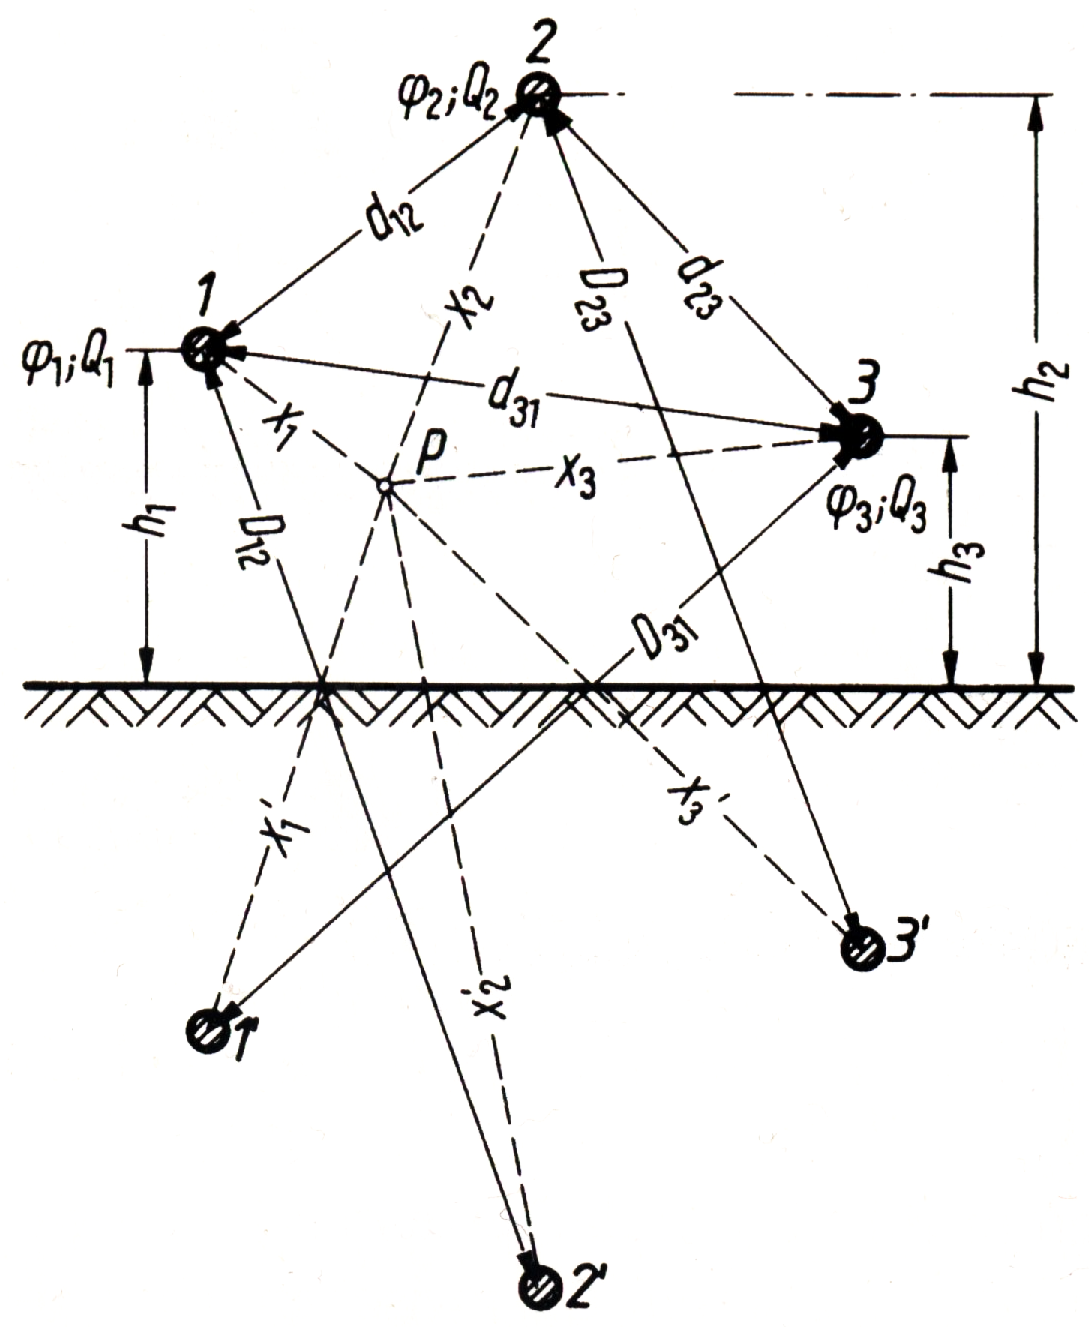
\includegraphics[scale=1]{gespiegelterdrehstrom.png}
\end{center}
\caption{bla} %fehlt
\end{figure}

 Die Kapazität einer Freileitung entsteht durch die die unterschiedlichen Potentiale der Leiterseil gegeneinander und gegenüber dem Erdpotential. Die Potentialunterschiede führen zu einem Elektrischem Feld, bestehend aus den elektrischen Flüssen $\Psi_{ij}$ zwischen zwei Leiterseilen, sowie den Flüssen $\Psi_{i0}$ zwischen je einem Leiter und dem Erdpotential. Zu jedem dieser Elektrischen Flüsse gehört eine Kapazität (Teilkapazität), welche zusammen die Kapazität der Freileitung ergeben.
Wir betrachten zunächst nur einen Leiter. Zur Berechnung der Kapazität verwenden wir Spiegelladungen: Wir ersetzen den Grund durch eine an der Erdoberfläche gespiegelte Ladung mit entgegengesetzter Ladung $Q'_1 = - Q_1$, ohne das sich das Feld ändert. Nun können wir das Potential in einem beliebigen Punkt P Als Summe der Potentiale schreiben:
\begin{equation}
\varphi = \frac{Q_1}{2\pi\varepsilon_0} \int^{x_1}_{r_1} \frac{dx_1}{x_1} + \varphi_1 + \frac{Q'_1}{2\pi\varepsilon_0} \int^{x_1}_{r_1} \frac{dx'_1}{x'_1} + \varphi'_1
\end{equation}
Wobei $r_1$ der Radius der Leiter ist, welche wir im folgenden als klein im Vergleich zu den Leiterabständen betrachten. Mit $Q'_1 = - Q_1$ und $\varphi'_1 = - \varphi_1$ ergibt sich:
\begin{equation}\label{einleitungsfeld}
\varphi = \frac{Q_1}{2\pi l\varepsilon_0} \ln \frac{x'_1}{x_1}
\end{equation}
An der Oberfläche des Leiters ist das Potential somit näherungsweise:
\begin{equation}
\varphi^* = \frac{Q_1}{2\pi l\varepsilon_0} \ln \frac{2h_1}{r_1}
\end{equation}
Dies entspricht aus auf Grund der Stetigkeit des Potentials % echt?
dem Potential des Leiters $\varphi_1 = \varphi^*$.
Betrachten wir nun ein System mit mehreren Leitern. Das Potential an einem wieder frei gewähltem Punkt P berechnet sich als die Summe der nach (\ref{einleitungsfeld}) berechneten Potentiale:
\begin{equation}
\varphi = \sum \frac{Q_i}{2\pi l\varepsilon_0} \ln \frac{x'i}{x_i}
\end{equation}
Wie zuvor setzen wir die Ortskoordinaten der Leiteoberflächen ein um die Potentiale der Leiter zu bestimmen, dadurch erhalten wir:
\begin{align}
\varphi_1 &= a_{11} Q_1 + a_{12} Q_{2} + ... + a_{1n} Q_n \\
\varphi_2 &= a_{21} Q_1 + a_{22} Q_{2} + ... + a_{2n} Q_n \\
\vdots \\
\varphi_n &= a_{n1} Q_1 + a_{n2} Q_{2} + ... + a_{nn} Q_n
\end{align}
mit den Koeffizienten
\begin{equation}
a_{ii} = \frac{\ln 2h_i/r_i}{2\pi l \varepsilon_0} \quad \textrm{und} \quad a_{ik} = \frac{\ln D_{ik}/d_{ik}}{2\pi l \varepsilon_0}
\end{equation}
Das obige Gleichungssystem muss nun nach den $Q_i$ aufgelöst werden. Das Gleichungssystem lässt sich auch in Matrizenschreibweiße $\boldsymbol{\varphi} = \uuline{A} \cdot \mathbf{Q}$ darstellen, dann entspricht das Auflösen der Invertierung der Matrix $\uuline{A}$: $\uuline{D}=\uuline{A}^{-1}$. Man erhält also allgemein:
\begin{equation}
Q_i = \sum_k d_{ik}\varphi_k
\end{equation}
Wir ziehen das Element mit $k=i$ aus der Summe hinaus und ergänzen:
\begin{equation}
Q_i = \sum_{k\neq i} d_{ik}\varphi_k + d_{ii}\varphi_i + \textcolor{blue}{\sum_k d_{ik}\varphi_i} - \textcolor{blue}
{\sum_k d_{ik}\varphi_i}
\end{equation}
Durch umsortieren und ausklammern erhalten wir schließlich eine Form in welcher wir die Teilkapazitäten identifizieren können.
\begin{equation}
Q_i = \underbrace{\left(d_{ii}+\sum_{k\neq i}d_{ik}\right)}_{:=C_{i0}}\varphi_i + \sum_{k\neq i} \underbrace{d_{ik}}_{:=C_{ik}} \left( \varphi_k - \varphi_i \right)
\end{equation}
Mithilfe der Regeln zur Parallel- und Reihenschaltung von Kondensatoren lässt sich daraus der Gesamtkapazitätsbelag berechnen.
Für eine Wechselstromleitung mit zwei Leiterseilen erhält man gemäß dieser Vorgehensweise\footnote{Dabei schrumpft das Gleichungssystem jedoch auf zwei Gleichungen zusammen, weshalb die Auflösung sehr einfach wird.}
\begin{equation}
C' = \frac{C}{l} = \frac{\varepsilon_0\pi}{\ln{\frac{2hd}{r\sqrt{\left(2h\right)^2+d^2}}}}
\end{equation}
Für eine Dreiphasenleitung ohne Erdleiter kann man man die Herleitung vereinfachen indem man ausnützt, dass die Ladungen der drei Leitungen zusammen immer Null ergeben. Möchte man jedoch, z. Bsp. für  Erdschlussstromberechnungen nicht nur die Gesamtkapazität sondern auch die einzelnen Teilkapazitäten berechnen, geht man nach dem beschriebenen Ansatz vor.
Da die Koeffizienten $a_{ii}$ und somit auch die Koeffizienten $d_{ik}$ von der Höhe der Leitungen über dem Erdboden abhängen, ergibt sich -- im Gegensatz zur Induktivität -- bei einer symmetrischen Dreiecksanordnung wie oben %verwais
unterschiedliche Kapazitäten für die Leitungen. Daher verdrillt man auch derartige symmetrische Leiter. Für einen derartigen Leiter erhält man den Kapazitätsbelag
\begin{equation}\label{verdrillteindukt}
C' = \frac{2\pi\varepsilon_0}{\ln\left(2 \bar{h}\bar{d}/(r\bar{D})\right) } \approx
\frac{2\pi\varepsilon_0}{\ln\left(\bar{d}/r\right)}
\end{equation}
Wobei $\bar{h}$, $\bar{d}$ und $\bar{D}$ die geometrischen Mittelwerte der Leiterhöhen, -Abstände und der Abstände zwischen einer Leitung und einer anderen \q Spiegelleitung\q : % Anführungszeichen fixen
\begin{equation}
\bar{h} := \sqrt[3]{h_1h_2h_3}, \quad \bar{d} := \sqrt[3]{d_{12}d_{23}d_{31}} \quad \bar{D} := \sqrt[3]{d_{12'}d_{23'}d_{31'}} \approx 2\bar{h}
\end{equation}
Man kann zeigen, dass ein zusätzliches Erdseil die Erdkapazität erhöht und die die Leiterkapazität verringert, so dass die Gesammtkapaziät unverändert bleibt und Gleichung (\ref{verdrillteindukt}) bleibt gültig.\cite{Flosdorff}


\subsubsection{Kabel}
In urbanen Gegenden sowie in Gegenden mit besonders erhaltenswerten Landschaften, setzt man statt Freileitungen auf unter der Erde verlegt Kabel. Die Leiter sind in der Regel aus Kupfer oder Aluminium und mit Ölimpregniertem Ölband oder neuer mit speziellen Kunststoffen isoliert. % flüssigkeitsimprägniertem Polypropylen/Papier-Laminat isoliert.
Neben Kosten und Gewichtseinsparungen haben moderne Kunststoffisolierungen auch elektrische Vorteile, so haben Kabel mit flüssigkeitsimprägniertem Polypropylen/Papier-Laminat eine um 67\% niedrigere dielektrische Verluste und eine 20\% niedrigere Permittivität und somit Kapazität.\cite{Harrison} Dadurch lässt sich mehr Leistung übertragen und es muss weniger Blindleistung bereitgestellt werden.
%Gaskablenm Druckgaskabel, (Druck-)Ölkabel
PVC-Kabel werden in Niederspannungs- und Mittelspannungsnetzen bis 10 kV eingesetzt. Für Hochspannungsnetze ist es wegen der hohen dielektischen Verluste ungeeignet, hier kommen neben Ölkabeln und Druckgaskabeln neuerdings Kabel mit vernetztem Polyäthylen (VPE) zum Einsatz. VPE hat hervorragende dielektrische und thermische Eigenschaften, weshalb es immer mehr in den Mittel und Niederspannungsbereich vordringt.\cite{Flosdorff}

\begin{figure}[tbhn]
\begin{center}
\noindent
\label{Ersatzschaltbildkabel}
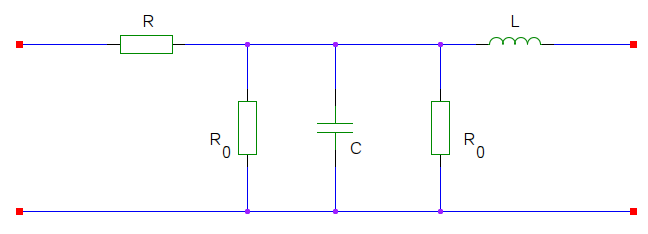
\includegraphics[scale=0.5]{kabel.png}
\end{center}
\caption{Ersatzschaltbild eines Kabels} %mehr
\end{figure}

% höhere Kosten, nidrigere Zuverlässigkeit
Das Ersatzschaltbild sieht wie das der Freileitung aus, nur das man zwei Parallel geschaltete Ableitungswiederstände betrachtet.
$R_0$ ist der Isolationswiederstand, während $R_d$ die dielektrischen Verluste beschreibt. Das sind Verluste die durch Polarisationseffekte im Dielektrikum der Kapazität entstehen.
Die Induktivitäten von Kabeln lassen sich nach den selben Gleichungen berechnen, wie die von Freileitungen, da hier Herleitung dieser ohne die Bedingung $d\gg r$ auskommt.\footnote{Dabei ist $\mu_0$ natürlich durch $\mu_r\mu_0$ – mit $\mu_r$ als der relativen Permeabilität des Materials – zu ersetzen} %was ist mit h>>d ?
Da bei Kabel die Leiterabstände deutlich kleiner sind sind auch die Induktivitäten kleiner: sie betragen nur etwas 25\% bis 30\% derWerte von Freileitungen\cite{Flosdorff}.
Die Berechnung der Kapazität von Kabeln, insbesondere Gürtelkabeln, ist ungleich schwieriger als bei Freileitern, da wir vorausgesetzt haben, dass $d\gg r$ ist auserdem sind die Dielektriken und der kreisförmige Metallmantel rechnerisch nur näherungsweise bestimmbar. Daher werden die Kapazitäten experimentell vom Hersteller bestimmt.\cite{Flosdorff}
Typische Werte für ein einphasiges Kupferkabel findet man in Tabelle \ref{fehlt}.
Wie wir mit den Werten feststellen können, ist bei Kabeln die Kapazität überwiegend,
besonders stark ist dies bei Unterseekabeln ausgeprägt. % überprüfen, warum?, Werte
Dazu kommt, dass bei Unterseekabeln die Blindleistungskompensation nur schwer möglich ist.
Die hohen Kapazitäten erfordern hohe Ströme zum Laden der Kapazität (Ladeströme), welche durch den gesamten zur Verfügung gestellten Strom aufgebracht werden müssen. Dies reduziert die übertragbare Leistung und führt ab einer gewissen Länge dazu, dass der maximal übertragbare Strom als Ladekapazität benötigt wird. % versteh ich selbst nur halb...
Für ein 400-kV-Kabel wie in Tabelle \ref{fehlt} liegt diese Länge bei 43,6 km.
Daher werden bei längeren Kabeln alle paar Kilometer % wieviel genau, besser formulieren…
Induktivitäten angeschlossen um die Blindleistung zu kompensieren.

\subsection{Netzregelung}
Elektrische Netze leiten elektrische Energie, können aber weder Energie erzeugen noch speichern.
Aufgrund der Energieerhaltung muss zu jedem Zeitpunkt exakt die gleiche Menge an Wirk- und Blindleistung in das Netz eingespeist werden, wie – einschließlich aller Verluste – verbraucht wird.
Es stellt sich daher die Frage, wie dies gewährleistet werden kann und was geschieht wenn dies für kurze Zeit nicht der Fall ist – den schließlich kann man aus unerwartete Veränderungen des Verbrauchs nicht beliebig schnell reagieren.

\subsubsection{Leistungs-Frequenz-Regelung}
Zunächst betrachten wir die Wirkleistung in einem Drehstromnetz, dass von Kraftwerken mit dampfgetriebenen Turbinen gespeist wird. Das Kraftwerk kann dabei ein Kohle-, Öl- oder Kernkraftwerk sein. \footnote{Statt diesen dampfgetriebenen Turbinen lassen sich auch Wasser- oder Windkraftwerke annehmen, lediglich Turbinenlose Kraftwerke wie Photovoltaikanlagen sind hierfür ungeeignet} % Gaskraftwerke?
Neben den Kraftwerken gibt es auch zahlreiche Drehstrommotoren auf der \q Verbraucherseite\q. % Anführungszeichen
In den Turbinen, Generatoren und Motoren rotieren Massen – darin ist Rotationsenergie gespeichert.
Steigt nur der Wirkleistungsverbrauch über die Menge an produzierter Wirkleistung, so wird die Energiedifferenz aus der Rotationsenergie der Maschinen entnommen.\cite{Harrison}
Dadurch wird deren Rotation jedoch langsamer – was zu einer Verringerung der Netzfrequenz führt.
Ist der Wirkleistungsverbrauch geringer als die Produktion, so geht die überschüssige Energie in Rotationsenergie der Maschinen über und die Netzfrequenz steigt.
In den Kraftwerken erkennt nun ein Sensor die Änderung der Frequenz und regulieren die Dampfventile entsprechend:
ist die Frequenz zu niedrig, wird mehr Dampf in die Turbinen gelassen, ist die Frequenz zu hoch, wird die Dampfzufuhr reduziert.
Man hält dadurch die Frequenz immer ungefähr konstant: in Großbritannien beträgt die Frequenz im Allgemeinen $50 \mathrm{Hz} \pm 0,05 \mathrm{Hz}$.\cite{Harrison} %Wert für Deutschland
%Details; auch in DE; alternativen?

\subsubsection{Blindleistungs-Spannungsregelung}
In einem elektrischen Netz muss nicht nur die bereitgestellte Wirkleistung gleich der produzierten sein, selbiges gilt auch für die Blindleistung.
Betrachtet man eine Last, die von einem Generator über eine Leitung mit ohmschen Widerstand und Blindwiderstand mit Leistung versorgt wird. Da auch an der Leistung eine Spannung abfällt, existiert eine Differenz zwischen der Generatorspannung und der an der Last anliegenden Spannung. Diese Differenz ist auch von der Blindleistung abhängig. Steigt also der Blindleistungsbedarf plötzlich, so steigt auch die Spannungsdifferenz und die Spannung an der Last sinkt. Dadurch sinkt wiederum der Blindleistungsbedarf – aber auch der Wirkleistungsbedarf.
Als Zahlenbeispiel sei genannt, dass eine Reduktion der Spannung um 1\% im gesamten Britischen Netz die Nachfrage nach Blindleistung um 5\% und die Nachfrage nach Wirkleistung um 1,4\% senken würde.
%Spannungsänderung duch stufensteller - was hat das damit zu tun?
%Bevor wir uns überlegen, wie dies gewährleistet wird,
Nun wollen wir ein paar Worte zur Erzeugung und "Vernichtung" von Blindleistung zum Ausgleich der von Verbrauchern und Leistungen erzeugten Blindleistung verlieren. Die wichtigste Rolle spielen dabei Synchrongeneratoren und Synchron-Phasenschieber.
Ist der Generator überangeregt, % erklären was das ist.
so erzeugt er Blindleistung, ist er unterangeregt, so nimmt der Blindleistung auf. Größe Synchrongeneratoren können bis zu 50\% ihrer Bemessungsleistung in Form von Blindstrom bereitstellen. %formulierung
Jedoch darf die aufgenommene Blindleistung nur bis zu 15\% detragen, wenn gleichzeitig die volle Wirkleistung erzeugt werden soll.\cite{Harrison}	%formulierung, so korrekt?, warum
Bei Synchron-Phasenschieber handelt es sich um im Leerlauf betriebene Synchronmotoren, deren Erregung automatisch durch die Spannung geregelt werden. Sie nehmen nur geringe Wirkleistung auf um ihre Verluste aus zu gleichen. Ein Gasturbinen-Generator kann – wenn keine Wirkleistung erzeugt werden soll – bei geeigneter Bauart von seiner Turbine abgekoppelt werden und dann als Synchron-Phasenschieber betrieben werden.\cite{Harrison}

Blindleistung kann auch durch parallelgeschaltete Kapazitäten erzeugt werden, diese haben jedoch den Nachteil das ihre Blindleistung proportional zu $U^2$ ist – sie also genau dann wenn man sie am dringendsten braucht weniger Blindleistung bereitstellen.\cite{Harrison}

\subsubsection{Gleichstrom-Netzregelung}
Die Regelung einer Gleichstromleitung ist weniger einfach, es wurden jedoch technische Möglichkeiten gefunden, eine HGÜ-Leitung äußerst schnell zu regeln. Auf diese wollen wir jedoch hier nicht eingehen, da sie eine umfangreiche Beschäftigung mit den technischen Details der Stromrichterstationen erfordern würden. % mehr

\section{Vor- und Nachteile der HGÜ gegenüber DHÜ}
Wir haben nun die physikalischen Grundlagen der elektrischen Energieübertragung kennengelernt, wir wollen nun die Vor und Nachteile beider Ansätze vergleichen und dabei auch technische und wirtschaftliche Aspekte berücksichtigen.

Gleichstrom hat den Nachteil, dass es im Gegensatz zum Wechselstrom keine einfache Möglichkeit der Lastflusssteuerung gibt.
Außerdem gibt es keine leistungsfähigen Gleichstrom-Schalter – das Betreiben von vermaschten Leitungen ist jedoch ohne leistungsfähige Schalter kaum möglich.\cite{Schymroch} % und ohne ordentliche Regelung auch nicht
Und während bei DHÜ an jeder Stelle einer Leitung das Entnehmen von Leistung mit einem simplen Transformator möglich ist braucht man bei HGÜ dafür komplexe Stromrichterstationen.\cite{Schymroch}
Daher ist und bleibt der Einsatz von HGÜ bis aus weiteres auf Punkt-zu-Punkt-Verbindungen beschränkt. Es gib nur wenige Ausnahmen, in welchen eine Verbindung von 3 Punkten mit Gleichstrom erfolgt ist. %wo, Quelle
Da es für unsere Bedürfnisse wichtig ist ein stark vernetztes Energienetz zu haben, muss die Grundstruktur %Wort
unserer Energienetze weiterhin auf Drehstrom basieren.

An den Enden einer solchen HGÜ-Leitung findet man jeweils eine Stromrichterstation, welche Transformatoren, Stromrichter, Filter und Regelungstechnik enthalten.\cite{Schymroch} In diesen Stationen wird auf der einen Seite der Wechselstrom in Gleichstrom umgewandelt, auf der anderen Seite dieser wieder in Wechselstrom zurück gewandelt.
% mehr zu funktionsweiße
Diese Stromrichterstation sind äußerst komplex und dadurch teuer und anfällig für Störungen. Auch haben sie vergleichsweiße hohe Verluste und benötigen Blindleistung, die von den angebundenen Netzen aufgebracht werden muss.

Die Leitung selbst haben jedoch geringere Verluste, was zum einen am nicht vorhandenen Skineffekt liegt, vor allem aber daran, dass nur Wirkleistung übertragen wird, in Gleichung \ref{Verlust} das $\varphi=0$ ist. Ab einer gewissen Länge sind HGÜ-Leitungen also effektiver als DHÜ-Leitungen.
Auch die Kosten für die Leitungen sind wesentlich geringer, dies liegt zum einen daran, dass man bei Drehstrom drei Leiter braucht, bei Gleichspannung jedoch mit zwei und bei Rückleitung über die Erde sogar nur mit einem Leiter auskommt. Dies spart Material und Bodenverbrauch. % Quelle, effizienz dadurch besser?
Dazu kommt, dass bei einer Drehstromleitung der Ausfall von nur einem Leiter zum Totalausfall der ganzen Leitung kommt, während eine Zweileiter-Gleichstrom-Leitung bei Ausfall eines Leiters noch mit halber Übertragungsleistung betrieben werden kann.\cite{Schymroch}\footnote{Allerdings wird die Rückleitung über die Erden nicht überall von den Behörden genehmigt.}%Quelle
Zum anderen sind die benötigen Leiter wesentlich einfacher. Dies hat einen ganze Reihe von Gründen:
Zunächst ist bei Gleichstrom die Effiktivspannung gleich der Maximalspannung, während bei Drehstrom die Maximalspannung um einen Faktor $\sqrt{2}$ höher ist und dss weiteren wird nur Wirk- und keine Blindleistung übertragen -- beide Effekte führen dazu, dass die Leitung nur auf eine niedrigere Spannungsfestigkeit ausgelegt werden muss. % Quelle
Bei Freileitungen mit Gleichstrom ist wie wir gesehen haben die Koronaentladung geringer, was nicht nur zu geringeren Verlusten führt, sondern vor allem dazu, dass man keine aufwendigen Bündelleiter benötigt.
Bei Kabeln, auf der anderen Seite, entfallen die Dielektrischen Verluste in der Isolierung und die Vorentladung ist wesentlich geringer, da es keine inhomogene Feldverläufe in den Isolierungen gibt. %genauer, Quelle

Gleichstromanlagen haben also sowohl was die Effizienz angeht also auch bezüglich der Wirtschaftlichkeit schlechte  Stromrichterstation, während die Leitung selbst effizienter und billiger ist als mit Drehstrom. Deshalb ist für kurze Leitungen Gleichstrom -- von Ausnahmen auf die wir unten zu sprechen kommen -- uninteressant, während für lange Leitungen die Vorteile überwiegen. Die Distanz ab der eine Gleichstromleitung wirtschaftlicher ist als eine Wechselstromleitung nennt man Break-Even-Distance, sie hängt von unterschiedlichen Parametern, insbesondere den Bodenpreisen und der Geländebeschaffenheit ab. %welche
\cite{Schymroch} beziffert die Break-Even-Distance für Freileitungen auf 300 km bis 700 km. %andere Quellen
Neben den teureren Leitungen und dem höheren Verlusten haben lange Drehstromleitungen noch ein weiteres Problem: ab einer gewissen Länge ist es nicht nur wegen den Verlusten, sondern auch aus Stabilitätsgründen, nötig die Blindleistung schon an Zwischenstationen zu kompensieren -- wir erinnern uns zum Beispiel daran, dass wir gesehen haben, dass ab einer gewissen Länge die Ladeströme die Leitungsströme übersteigen. Da die Kapazitiver Blindleistung eines Kabels wesentlich höher als die Induktivität einer Freileitung ist, ist die Länge, ab welche eine Blindleistungskompensation unterwegs erforderlich ist, bei Kabeln wesentlich geringer als bei Freileitungen %Wort.
Dies ist bei Unterseekabeln noch stärker, welche aufgrund der hohen Permittivität und Leitfähigkeit des Meereswassers eine noch höhere Kapazität haben. Bei Unterseekabeln ist die Blindleistungskompensation nicht nur teuer sonder sogar technisch kaum möglich. Daher sind auch kürzere Unterseekabel zwangsläufig Gleichstromleitungen. %Zahlen!
Die Länge einer Gleichspannungsleitung ist jedoch nur durch die ohmschen Verluste begrenzt.\cite{Schymroch}

Soll nun jedoch ein sogenanntes Drehstrom-Inselnetz -- also ein abgeschlossenes kleines Netz -- über eine HGÜ gespeist werden, wie es beispielsweise bei der schwedischen Insel Gotland geschieht, muss bedacht werden, dass die HGÜ-Leitung nur Wirkleistung transportiert. Die Blindleistung für das Inselnetz, wie auch für die Stromrichterstation muss Vor-Ort kompensiert werden.

Ein weitere Vorteil der sich aus dem Gleichstrom ergibt ist, dass die durch die Leitung verbunden Netzpunkte nicht Syncron sein müssen, sie können also einen Phasenunterschied zu einander oder sogar unterschiedliche Frequenzen haben. Damit könnten Netze mit unterschiedlichen Frequenzen (50 Hz oder 60 Hz) mit einander verbunden werden. So wurde in Sakuma, Japan das 50-Hz-Netz des Norden mit dem 60-Hz-Netz des Südens durch die HGÜ-Anlage Higashi-Shimizu mit einer Leitungslänge von nur wenigen Metern verbunden.\cite{Schymroch} %andere Quelle

%% kein Skineffekt
% Verschmutzungsbla -> WP
%% keine Phasenverscheibung durch abstand ? 
% hohe Geschw. der Regelung => kurzschluß-Strom gleich Nenstrom.


\section{Ein kurzer geschichtlicher Abriss und Ausblick}
Wir wollen auch einen kurzen Abriss der durchaus interessanten Geschichte der Energie"-übertragung mit Gleich- und Wechselspannung geben. Dabei beziehen wir uns bei der Geschichte bis in die 1980er Jahre primär auf \cite{Schymroch}.

Die Geschichte der elektrischen Energie begann 1882 auf der Internationalen Ausstellung in München – mit einer Gleichstrom-Anlage. Der französische Physiker Marcel Deprez übertrug einer elektrische Leistung von 1,4 kW von Miesbach nach München – also über 57 km – mit zwei einfachen Telegrafendrähten mit einer Spannung zwischen 1,5 kV und 2,0 kV. Die Demonstationsanlage betrieb in München die Pumpen eines Springbrunnens. Die Verluste der Anlage betrugen 78\%. Eine weitere Steigerung der Spannung auf 6 kV scheiterte an Isolationsschwierigkeiten beim Gleichstrom-Generator. Dieses Problem wurde 1884 von Lafontaine gelöst, indem mehrere von einander isoliert montierte Generatoren parallelgeschalten wurden und auch auf der Verbraucher-Seite wurden parallelgeschaltene Motoren verwendet. Dadurch konnte der Wirkungsgrad einer 50\ km langen Leitung auf 50\% erhöht und 70\ kW übertragen werden.

Auch nach Entdeckung des Transformators im Jahr darauf, wurde Wechselspannung -- obwohl sie sich verlustarm hochspannen ließ -- weiterhin nicht verwendet.
Dies ist auf den zur damaligen Zeit sehr renommierten italenischen Physiker Galileo Ferraris zurückführen,
der einen falschen, aber sehr überzeugenden Beweis erbrachte, dass Wechselspannungsübertragungen maximal einen Wirkungsgrad von nur 50\% erreichen können.
Da dem Beweis des berühmten Physikers glauben geschenkt wurde, wurde vorübergehend nicht an dem Thema weitergearbeitet.
Auch die Demonstration einer Drehstrom-Übertragung von Laufen nach Frankfurt auf der dortigen Weltausstellung im Jahr 1891 konnten die Favorisierung der Gleichstromübertragung nicht stoppen.
Der Schweizer Ingenieur René Thury -- auch bekannt als der König des Gleichstroms -- hatte ein wirksames und zuverlässiges Regelungssystem für die in Reihe geschalteten Generatoren und Motoren entwickelt, so dass Gleichstrom mit Spannungen von bis zu 180\ kV übertragen werden konnte. In den nächsten zwanzig Jahren wurden 15 Übertragungen nach dem Prinzip von Thury gebaut. Das letzte dieser Anlagen und gleichzeitig auch das letzte Gleichspannungssystem mit mechanischen Wandlern war die Anlage zwischen Moutiers und Lyon, sowie später den Zwischenstationen Rosiers und Vignotanne. Sie Übertrug zunächst 4,5\ MW und nach einem Ausbau 14\ MW Leistung. Die Anlage bestand aus drei Kraftwerken und zwei Verbraucherstationen (eine eigene für die Straßenbahnen), war also vergleichsweise komplex. Die Anlage wurde 1937 zugunsten einer, der ab 1930 als überlegen angesehenen, DHÜ-Systeme demontiert. Die Idee der HGÜ geriet jedoch nicht in Vergessenheit, da zu jener Zeit mit den Stromrichtern die Grundlage für moderne Stromrichterstationen erfunden wurde.

Die ersten Versuchsanlagen mit, auf Thyratron-Stromrichtern, basierenden Quecksilberdampfgleichrichtern wurden in den USA entwickelt, wo 1936 eine erste 26\ km lange Versuchsanlage mit einer Leistung von 5,25\ MW bei einer Nennspannung von 30\ kV errichtet wurde. Sie wurde zwischen zwei Netzen mit unterschiedliche Frequenz (40\ Hz und 60\ Hz) gebaut um zu demonstrieren, dass die Netze nicht synchron sein müssen. Die erste Versuchsanlage in Deutschland wurde 1944 als Zwei-Leiter-Anlage mit Spannungen von $\pm 200 kV$ von der AEG und Siemens gebaut und hatte eine Leistung von 60\ MW. Nach dem Krieg wurde die Anlage von russischen Ingenieuren demontiert und zwischen Kashira und Moskau als Ein-Leiter-Versuchsanlage wieder aufgebaut.

\newpage

Die erste kommerziell betriebene Anlage ist die schon angesprochene Anlage zur vollständigen Wirkleistungsversorgung der Insel Gotland mit einem 20 MW-Seekabel mit der Spannung von --100\ kV.

Seit Beginn der 1970er Jahre wurden die Thyratron-Gleichrichter durch ihre halbleiteräquivalenten, den Thyristoren ersetzt. Die letzte mit Thyratrons gebaute Anlage war die englische HGÜ Kingsnorth. Thyristor-Technologie wird bis heute bei HGÜ-Stromrichtern verwendet, jedoch kam ab 1997 die IGBT-Technik (Bipolartransistor mit isolierter Gate-Elektrode) als Alternative hinzu. Derartige Anlagen werden oft auch unter den Namen HVDC light oder HVDC plus vertrieben.
Während die Leistung von IGBT-basierten Anlagen auf deutlich unter 1.000 MW beschränkt ist, gibt es bereits Thyristor-Anlagen mit Leistungen von bis zu 6.400\ MW:
Die chinesische HGÜ Xianjiaba-Shanghai wurde 2010 fertiggestellt.\cite{Kao}
Sie transportiert eine Leistung von 6.400\ MW bei einer Spannung von $\pm800 kV$ über 2071 Kilometer und
soll nur die erste von 12 bis 2018 fertiggestellten derartig dimensionierten Gleichstrom-Leitungen in China sein.\cite{Liste}
Die Längen der HGÜ-Leitungen betragen bis zu 2.400 Kilometer bei Freileitungen und bis zu 700\ km bei Kabeln.\cite{Liste} 

\begin{figure}[hbtn]
\begin{center}
\noindent
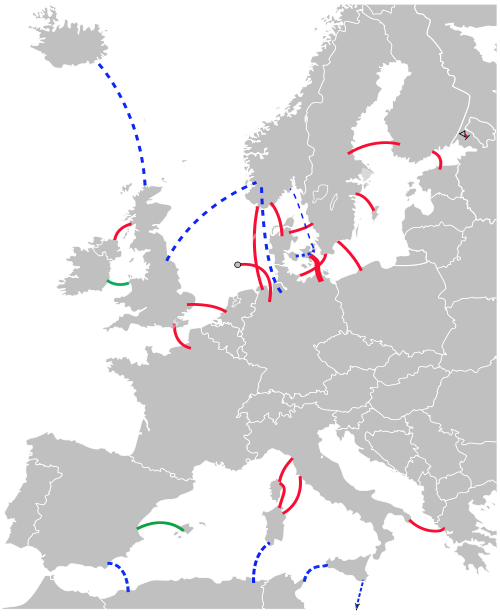
\includegraphics[scale=0.55]{HVDC_Europe.png}
\end{center}
\caption{HGÜ-Leitungen in Europa -- Rot: bestehend, Grün: in Bau; Blau: geplant. Quelle: \cite{Europa}}
\label{pic:Europa}
\end{figure}

In Europa ist der Einsatz von HGÜ jedoch immer noch fast ausschließlich auf Seekabel beschränkt -- auf allen anderen Kontinenten (natürlich ausgenommen der Antarktis) gibt es hingegen auch lange gleichstrombetriebene Freileitungen:

So wurde bereits 1979 die 1.410 Kilometer lange HGÜ-Freileitung \q Cahora Bassa\qe zwischen der Cahora Bassa-Talsperre im Norden von Mosambik und dem Großraum um Johannesburg in Südafrika fertiggestellt (Spannung: $\pm$533\ kV; Leistung: 1.920\ MW)
und im gleichen Jahr wurde auch eine 1.770 Kilometer lange Freileitung \q Inga Shaba\qe in der heutigen Demokratische Republik Kongo (Spannung: $\pm$500\ kV; Leistung: derzeit 200\ MW, ausgelegt auf 560\ MW) errichtet\cite{Schymroch}.
Auch \q Inga Shaba\qe dient zur Verteilung von Energie aus einem Wasserkraftwerk (Inga-Staudammes),
bei ihr wurden für die Pole jeweils eine eigene Trasse gebaut und sie kann sowohl bipolar als auch mono- oder homopolar betrieben werden\cite{Schymroch}.
In Nordamerika existieren zahlreiche HGÜ-Anlagen, besonders hervorzuheben ist unter anderem die HGÜ Quebec–New England, welche zwei asynchrone Netze über 1.500 Kilometer mit einer Übertragungsleistung von 2,25 GW verbindet und dabei 3 Stromrichterstationen hat (Spannung: $\pm$450 kV; errichtet 1986, ausgebaut 1992)\cite{Liste}.
Die mit über 2.500 km weltweit längste Freileitung soll noch dieses Jahr in Brasilien fertig gestellt werden, auch sie ist eine der wenigen Leitungen die drei Punkte verbindet (Spannung: $\pm$600 kV; Leistung: 3.150 MW). %cite
In Neuseeland wird ein beträchtlicher Teil der Energie der Nordinsel mit der bereits 1965 errichteten und zahlreich um- und ausgebauten Leitung \q Inter-Island\qe von der Südinsel bezogen (Spannung: +270 kV, --350 kV; Leistung: 1.240 MW; Länge: 535 km Freileitung und 40 km Seekabel) \cite{Schymroch}\cite{Liste}.
In Asien setzen, wie auch schon angesprochen, vor allem China zahlreiche Gleichstromanlagen zum Ausbau des schnell wachsenden Stromnetzes ein, dies dürfte neben dem starken Wirtschaftswachstum auch in der enormen Größe des Landes begründet sein.

In den letzten Jahren erfuhr die HGÜ-Technik durch den Boom der erneuerbaren Energien einen neues Interesse, da diese zu stärkeren örtlichen und zeitlichen Unterschieden der Energieproduktion führen.
So ist zum Beispiel in Norddeutschland, im Vergleich zu Süddeutschland, ein sehr großes Potential an Windkraft verfügbar. Daher planen deutsche Netzbetreiber laut Berichten der FAZ und der Financial Times Deutschland HGÜ-Trassen von Magdeburg ins Rhein-Main-Gebiet, von Rheinland nach Baden-Württemberg und von Schleswig-Holstein nach Bayern.\cite{FAZ1}\cite{FAZ2}\cite{FinancialTimes}
Durch diesen Aufschwung ist der Begriff der Hochspannungs-Gleichstrom-Übertragung auch außerhalb der Fachwelt deutlich bekannter geworden.

Besonders wichtig wäre eine Gleichstromübertragung auch für das DESERTEC-Konzept, welches vorsieht, große Mengen an in afrikanischen Wüsten erzeugtem Ökostrom in die europäischen Energienetze einzuspeisen. Die Übertragung der Energie vom afrikanischem zum europäischem Kontinent wäre nur mit HGÜs sinnvoll umsetzbar und auch innerhalb Europas bräuchte es HGÜ-Leitungen um die Redundanz, Stabilität und Versorgungssicherheit des Netzes zu gewährleisten.\cite{TRANS-CSP}



%%% ---------------------------
% eifügen, wenn noch nicht klar:
%% Blindleistung in den Netzen niedrig halten, da Netztbelastung(Scheinleistung) => weniger Wirkleistung mögl.
% Leitungen: 6° Phasenverschiebung/100km
% Konverterstat. bruachen Blindleistung
% In England wird bei Laststößen die Spannung konstant gehalten und die Frequenz gibt nach, in festland-Europa andersherum
% Hohlleitungen auf für reduzierungs von Koronaentladung (Bergmann-Schaefer)
\FloatBarrier
\bibliography{lit}{}
\bibliographystyle{unsrtdin}
\renewcommand{\refname}{Literatur und Quellen}

%\listoffigures

\newpage
\tableofcontents

\end{document}
